\section{Chuyển đổi các cú pháp Rust sang đồ thị CPG}

Phần này sẽ trình bày một số cú pháp của Rust khác biệt so với ngôn ngữ C/C++ và cách mà công cụ đã chuyển đổi sang đồ thị CPG cho các cú pháp này.
Các cú pháp bao gồm: if let, while let, match, lifetime.
Những đoạn mã nguồn và hình ảnh mô tả đồ thị CPG được sử dụng từ giờ đến cuối khóa luận sẽ được đơn giản hóa để dễ dàng thể hiện và minh họa.
Các cạnh và các nút không phải trọng tâm của đồ thị CPG sẽ được loại bỏ để tập trung vào các tính năng cần trình bày.

\subsection{Cú pháp if let}
If else là cấu trúc điều khiển có mặt trong tất cả các loại ngôn ngữ phổ biến.
% Nó cho phép chúng ta kiểm tra một điều kiện và thực thi một khối mã nếu điều kiện đúng và một khối mã khác nếu điều kiện sai.
Cấu trúc câu lệnh if else sẽ bao gồm một điều kiện và 2 khối mã.
Nếu điều kiện đúng, khối mã trong if sẽ được thực thi, ngược lại khối mã trong else sẽ được thực thi.
Thông thường khối điều kiện sẽ là biểu thức trả về kết quả đúng hoặc sai của biểu thức đó.
Trong ngôn ngữ như C/C++ thì chỉ chấp nhận biểu thức điều kiện, việc sử dụng mệnh đề (có dấu hai chấm để kết thúc câu lệnh) là không hợp lệ.
Với phương châm "Expression over statement" và nhằm mục đích tạo sự ngắn gọn, Rust cho phép thực hiện phép khai báo biến và gán giá trị cho biến trong cùng một câu lệnh bằng điều kiện if let.
Cú pháp tổng quát của câu lệnh if let như sau:

\begin{listing}[H]
\begin{minted}[mathescape, breaklines, frame=lines, framesep=2mm, baselinestretch=1.2, fontsize=\footnotesize, linenos]{rust}
if let <pattern> = <expression> {
     <block>
} else {
     <block>
}
\end{minted}
\caption{Mã giả cho cú pháp tổng quát của if let.}
\label{code:c4_iflet_general}
\end{listing}

Cú pháp \ref{code:c4_iflet_general} sẽ thực hiện 2 công việc.
Thứ nhất là kiểm tra xem \texttt{<expression>} có khớp với \texttt{<pattern>} hay không, nếu không khớp thì trả về $false$, nếu khớp thì trả về $true$.
Thứ hai là khai báo các biến mới từ \texttt{<pattern>} nếu điều kiện thành công, các biến sẽ có phạm vi tồn tại trong khối lệnh điều kiện thành công.
% thì tiếp tục thực hiện tạo biến mới dựa theo \texttt{<pattern>}

\begin{listing}[H]
\begin{minted}[mathescape, breaklines, frame=lines, framesep=2mm, baselinestretch=1.2, fontsize=\footnotesize, linenos]{rust}
let number: Option<i32> = None;

if let Some(i) = number {
    println!("Matched number {:?}!", i);
} else {
    // ...
}
\end{minted}
\caption{Ví dụ đoạn mã nguồn cho cú pháp if let.}
\label{code:c4_iflet}
\end{listing}

Đoạn mã \ref{code:c4_iflet} sử dụng cú pháp if let với điều kiện là kiểm tra xem biến \texttt{number} có giá trị bên trong hay không, nếu có thì khai báo một biến \texttt{i} mới và gán giá trị cho biến \texttt{i}.
Tiếp theo sẽ thực thi khối lệnh bên trong if.
Biến \texttt{i} sẽ chỉ tồn tại trong khối lệnh if, và được sử dụng trong câu lệnh \texttt{println!}.
Do thực hiện 2 công việc trong cùng 1 câu lệnh nên khi quy đổi sang câu lệnh tương tự trong ngôn ngữ C/C++, cú pháp if let sẽ tương đương 2 câu lệnh kiểm tra điều kiện và gán biến \ref{code:c4_iflet_cpp}.

\begin{listing}[H]
\begin{minted}[mathescape, breaklines, frame=lines, framesep=2mm, baselinestretch=1.2, fontsize=\footnotesize, linenos]{cpp}
Object* obj = inputObj();

if (obj != nullptr) { // 1 câu lệnh kiểm tra điều kiện
    int number = *static_cast<int*>(obj); // 1 câu lệnh gán biến
    std::cout << "Matched " << number << "!" << std::endl;
}
\end{minted}
\caption{Ví dụ đoạn mã nguồn cho cú pháp if let tương đương trong C++.}
\label{code:c4_iflet_cpp}
\end{listing}

\begin{figure}[H]
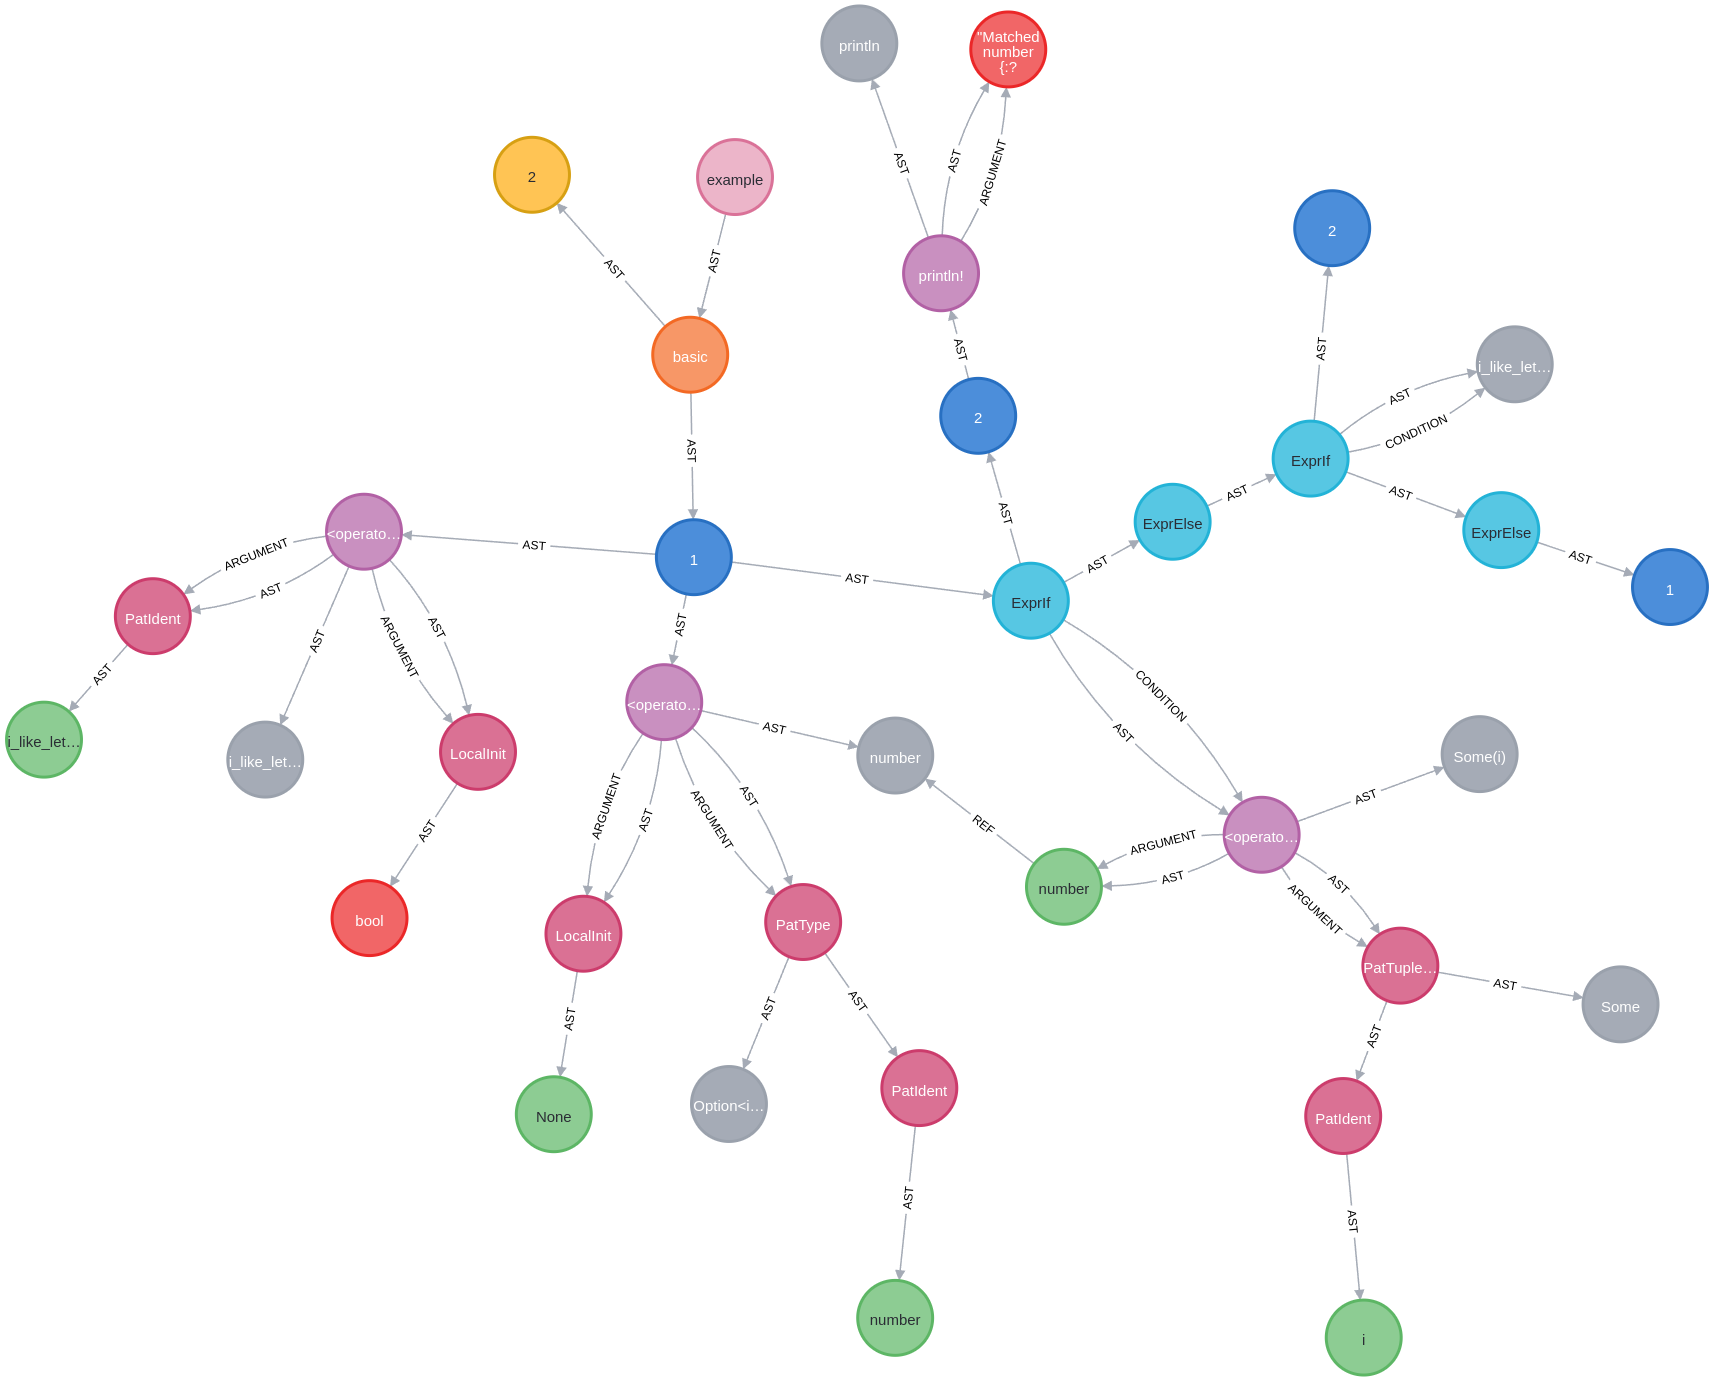
\includegraphics[width=1\columnwidth]{figures/c4/c4_iflet.png}
\centering
\caption{Minh họa đồ thị CPG cho đoạn mã nguồn cú pháp if let \ref{code:c4_iflet}.}
\label{img:c4_cpg_iflet}
\end{figure}

% Trong Hình \ref{img:c4_cpg_iflet}, cạnh \texttt{CONDITION} của nút \texttt{ExprIf} trỏ tới nút \texttt{Assignment}, đồng thời cũng khai báo biến mới với tên \texttt{i}. Mặc định, Joern sẽ không cho phép cạnh \texttt{CONDITION} trỏ tới nút \texttt{Assignment} bởi vì trong ngôn ngữ C/C++ không thể lấy một phép gán làm điều kiện. Tuy nhiên, khóa luận đã thực hiện chỉnh sửa đặc tả CPG của Joern để cho phép cạnh \texttt{CONDITION} trỏ tới nút \texttt{Assignment} trong trường hợp này.
% Điều chỉnh này giúp mô hình hóa chính xác hơn ngữ nghĩa của các ngôn ngữ hỗ trợ khai báo biến trực tiếp trong khối điều kiện, như Rust. Các mệnh đề trong khối điều kiện đúng được thực thi, nếu có sử dụng tới biến \texttt{i} thì sẽ tham chiếu tới biến \texttt{i} vừa được khai báo thông qua cạnh \texttt{REF}. Nhờ đó, đồ thị CPG không chỉ phản ánh chính xác cấu trúc mã nguồn mà còn đảm bảo khả năng truy vấn và phân tích đúng các phụ thuộc dữ liệu trong các ngữ cảnh tương tự.

Trong Hình \ref{img:c4_cpg_iflet}, cạnh \texttt{CONDITION} của nút \texttt{ExprIf} trỏ tới nút \texttt{Assignment}, đồng thời cũng khai báo biến mới với tên \texttt{i}.
Mặc định, Joern sẽ không cho phép cạnh \texttt{CONDITION} trỏ tới nút \texttt{Assignment} bởi vì trong ngôn ngữ C/C++ không thể lấy một phép gán làm điều kiện.
Tuy nhiên, khóa luận đã thực hiện chỉnh sửa đặc tả CPG của Joern để cho phép cạnh \texttt{CONDITION} trỏ tới nút \texttt{Assignment} trong trường hợp này.
Điều chỉnh này giúp mô hình hóa chính xác hơn ngữ nghĩa của các ngôn ngữ hỗ trợ khai báo biến trực tiếp trong khối điều kiện như Rust.
Các mệnh đề trong khối điều kiện đúng được thực thi, nếu có sử dụng tới biến \texttt{i} thì sẽ tham chiếu tới biến \texttt{i} vừa được khai báo thông qua cạnh \texttt{REF}.

\subsection{Cú pháp while let}

% Tương tự với tính năng if let ở trên, Rust cũng hỗ trợ việc khai báo biến làm điều kiện cho vòng lặp while.
% Cú pháp của vòng lặp while let như sau:

% \begin{minted}[mathescape, breaklines, frame=lines, framesep=2mm, baselinestretch=1.2, fontsize=\footnotesize, linenos]{rust}
% while let <pattern> = <expression> {
%         <block>
% }
% \end{minted}


\begin{listing}[H]
\begin{minted}[mathescape, breaklines, frame=lines, framesep=2mm, baselinestretch=1.2, fontsize=\footnotesize, linenos]{rust}
let mut optional = Some(0);

while let Some(i) = optional {
    if i > 9 {
        optional = None;
    } else {
        optional = Some(i + 1);
    }
}
\end{minted}
\caption{Ví dụ đoạn mã nguồn cho cú pháp while let.}
\label{code:c4_whilelet}
\end{listing}

Tương tự với cú pháp if let ở trên, Rust cũng hỗ trợ việc khai báo biến làm điều kiện cho vòng lặp while.
Đoạn mã \ref{code:c4_whilelet} trên được hiểu là nếu biến \texttt{optional} có giá trị bên trong thì thực hiện vòng lặp, nếu không thì kết thúc vòng lặp.
Đồng thời, sẽ có một biến \texttt{i} mới được khởi tạo đối với mỗi lần lặp, giá trị của \texttt{i} bằng giá trị của số nguyên bên trong biến \texttt{optional}.
Các mệnh đề trong khối được thực thi, và nếu có sử dụng tới, chúng sẽ tham chiếu tới biến \texttt{i} vừa được khai báo thông qua cạnh \texttt{REF}.
Không chỉ vậy, vế phải của điều kiện có thể được gán lại liên tục trong quá trình lặp, đảm bảo vòng lặp kiểm tra trạng thái mới của biến \texttt{optional} sau mỗi lần lặp.
Nhờ vậy thể hiện được các thay đổi động của dữ liệu trong suốt quá trình thực thi vòng lặp.
Khi việc kiểm tra giá trị số nguyên bên trong biến \texttt{optional} thất bại, vòng lặp sẽ kết thúc.
% , đảm bảo hành vi nhất quán với ngữ nghĩa của mã nguồn Rust.

Hình \ref{img:c4_cpg_whilelet} mô tả đồ thị CPG cho đoạn mã nguồn while let ở trên.
Nút \texttt{CONTROL STRUCTURE} thể hiện vòng lặp while, trong khi nút \texttt{ASSIGNMENT} biểu diễn điều kiện của vòng lặp và được nối với nút \texttt{CONTROL STRUCTURE} thông qua cạnh \texttt{CONDITION}
Ngoài ra, biến \texttt{i} được khai báo riêng tại nút \texttt{LOCAL} và tham chiếu thông qua cạnh \texttt{REF} bởi các nút tương ứng với các mệnh đề trong khối mã.

\begin{figure}[H]
    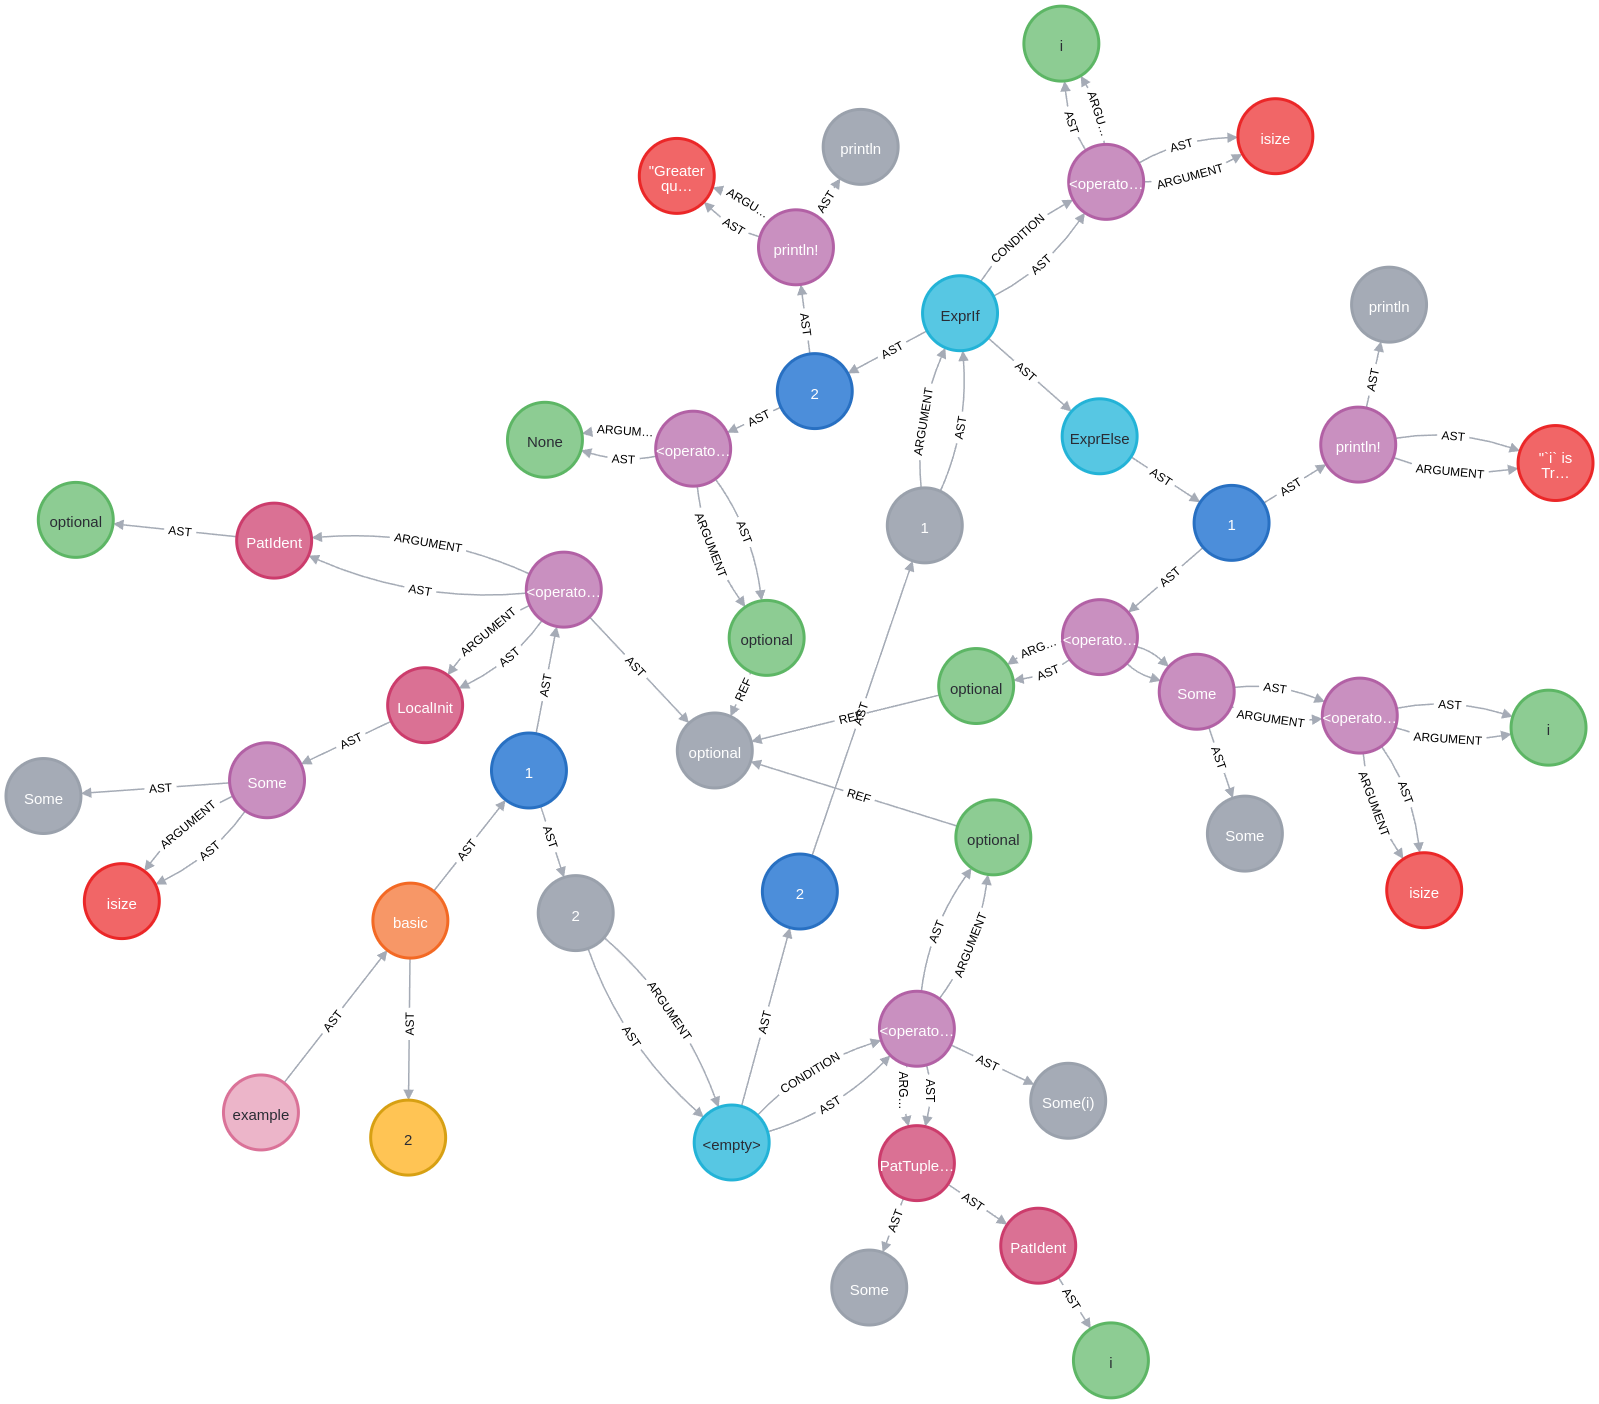
\includegraphics[width=1\columnwidth]{figures/c4/c4_whilelet.png}
    \centering
    \caption{Minh họa đồ thị CPG cho đoạn mã nguồn cú pháp while let \ref{code:c4_whilelet}.}
    \label{img:c4_cpg_whilelet}
\end{figure}

\subsection{Cú pháp match}

Ngoài việc sử dụng mệnh đề gán biến thành biểu thức điều kiện, tính hướng hàm của Rust còn thể hiện ở sự kết hợp giữa cơ chế pattern matching và kiểu dữ liệu đại số.
Đoạn mã \ref{code:c4_match} cho thấy cấu trúc match không chỉ kiểm tra giá trị mà còn kết hợp với các mẫu phức tạp, bao gồm kiểm tra điều kiện, kiểm tra các kiểu dữ liệu khác nhau và so sánh.
Điều này mang lại cho Rust tính linh hoạt cao hơn so với switch trong C/C++ khi chỉ so sánh giá trị nguyên thủy.
Một điểm khác biệt quan trọng giữa match và switch là tính toàn diện của match.
Rust yêu cầu các mẫu trong match phải bao quát tất cả các khả năng có thể xảy ra, nếu không trình biên dịch sẽ báo lỗi.
Điều này giúp đảm bảo rằng không có tình huống nào bị bỏ qua, tăng cường độ an toàn của mã nguồn.
Trong khi đó, switch trong C/C++ không yêu cầu bao quát tất cả các trường hợp, và việc bỏ sót một trường hợp có thể dẫn đến lỗi hoặc hành vi không mong muốn.
Thêm vào đó, match trong Rust cho phép trích xuất và xử lý các thành phần của cấu trúc dữ liệu phức tạp ngay trong quá trình đối chiếu mẫu.
% Ví dụ, Rust có thể match trên \texttt{tuple}, \texttt{enum}, \texttt{struct}, trong khi switch của C/C++ thường chỉ giới hạn trong các giá trị nguyên thủy.
Cú pháp match có thể thực hiện trên \texttt{tuple}, \texttt{enum}, \texttt{struct}, trong khi switch của C/C++ chỉ giới hạn cho các giá trị nguyên thủy.

\begin{listing}[H]
\begin{minted}[mathescape, breaklines, frame=lines, framesep=2mm, baselinestretch=1.2, fontsize=\footnotesize, linenos]{rust}
enum Color {
    Red,
    Blue(u32, u32, u32),
    Green {
        red: u32,
        green: u32,
        blue: u32
    },
}

fn main() {
    let color = Color::Blue(0, 0, 255);
    match color {
        Color::Red =>
            println!("The color is Red!"),
        Color::Blue(r, g, b) =>
            println!("R: {}, G: {}, B: {}!", r, g, b),
        Color::Green { red, green, blue } => {
            println!("Red: {}, Green: {}, Blue: {}!", red, green, blue)
        }
    }
}
\end{minted}
\caption{Ví dụ đoạn mã nguồn cho cú pháp match.}
\label{code:c4_match}
\end{listing}

Trong Hình \ref{img:c4_match}, các biến thể của \texttt{enum Color} được thể hiện bằng nút \texttt{VARIANT}.
Biến thể \texttt{Red} do không có giá trị nên không có nút con nào khác.
Biến thể \texttt{Blue} có giá trị là 3 số nguyên tính theo chỉ mục nên sẽ có 3 nút con \texttt{MEMBER} tương ứng, nhưng mỗi nút \texttt{MEMBER} này không có nút con \texttt{IDENTIFIER} chỉ ra tên thành phần.
Ngược lại mỗi nút \texttt{MEMBER} của \texttt{Green} sẽ có nút con \texttt{IDENTIFIER} thể hiện tên của thành phần.
Còn cú pháp match được thể hiện bằng nút \texttt{CONTROL STRUCTURE} và cạnh \texttt{CONDITION} nối với nút \texttt{IDENTITER} chỉ tới biến \texttt{color}.
Mỗi trường hợp của match sẽ được thể hiện bằng nút \texttt{ARM} và mỗi \texttt{ARM} cũng có sẽ cạnh \texttt{CONDITION} nối tới nút thể hiện biểu thức điều kiện.

\begin{figure}[H]
    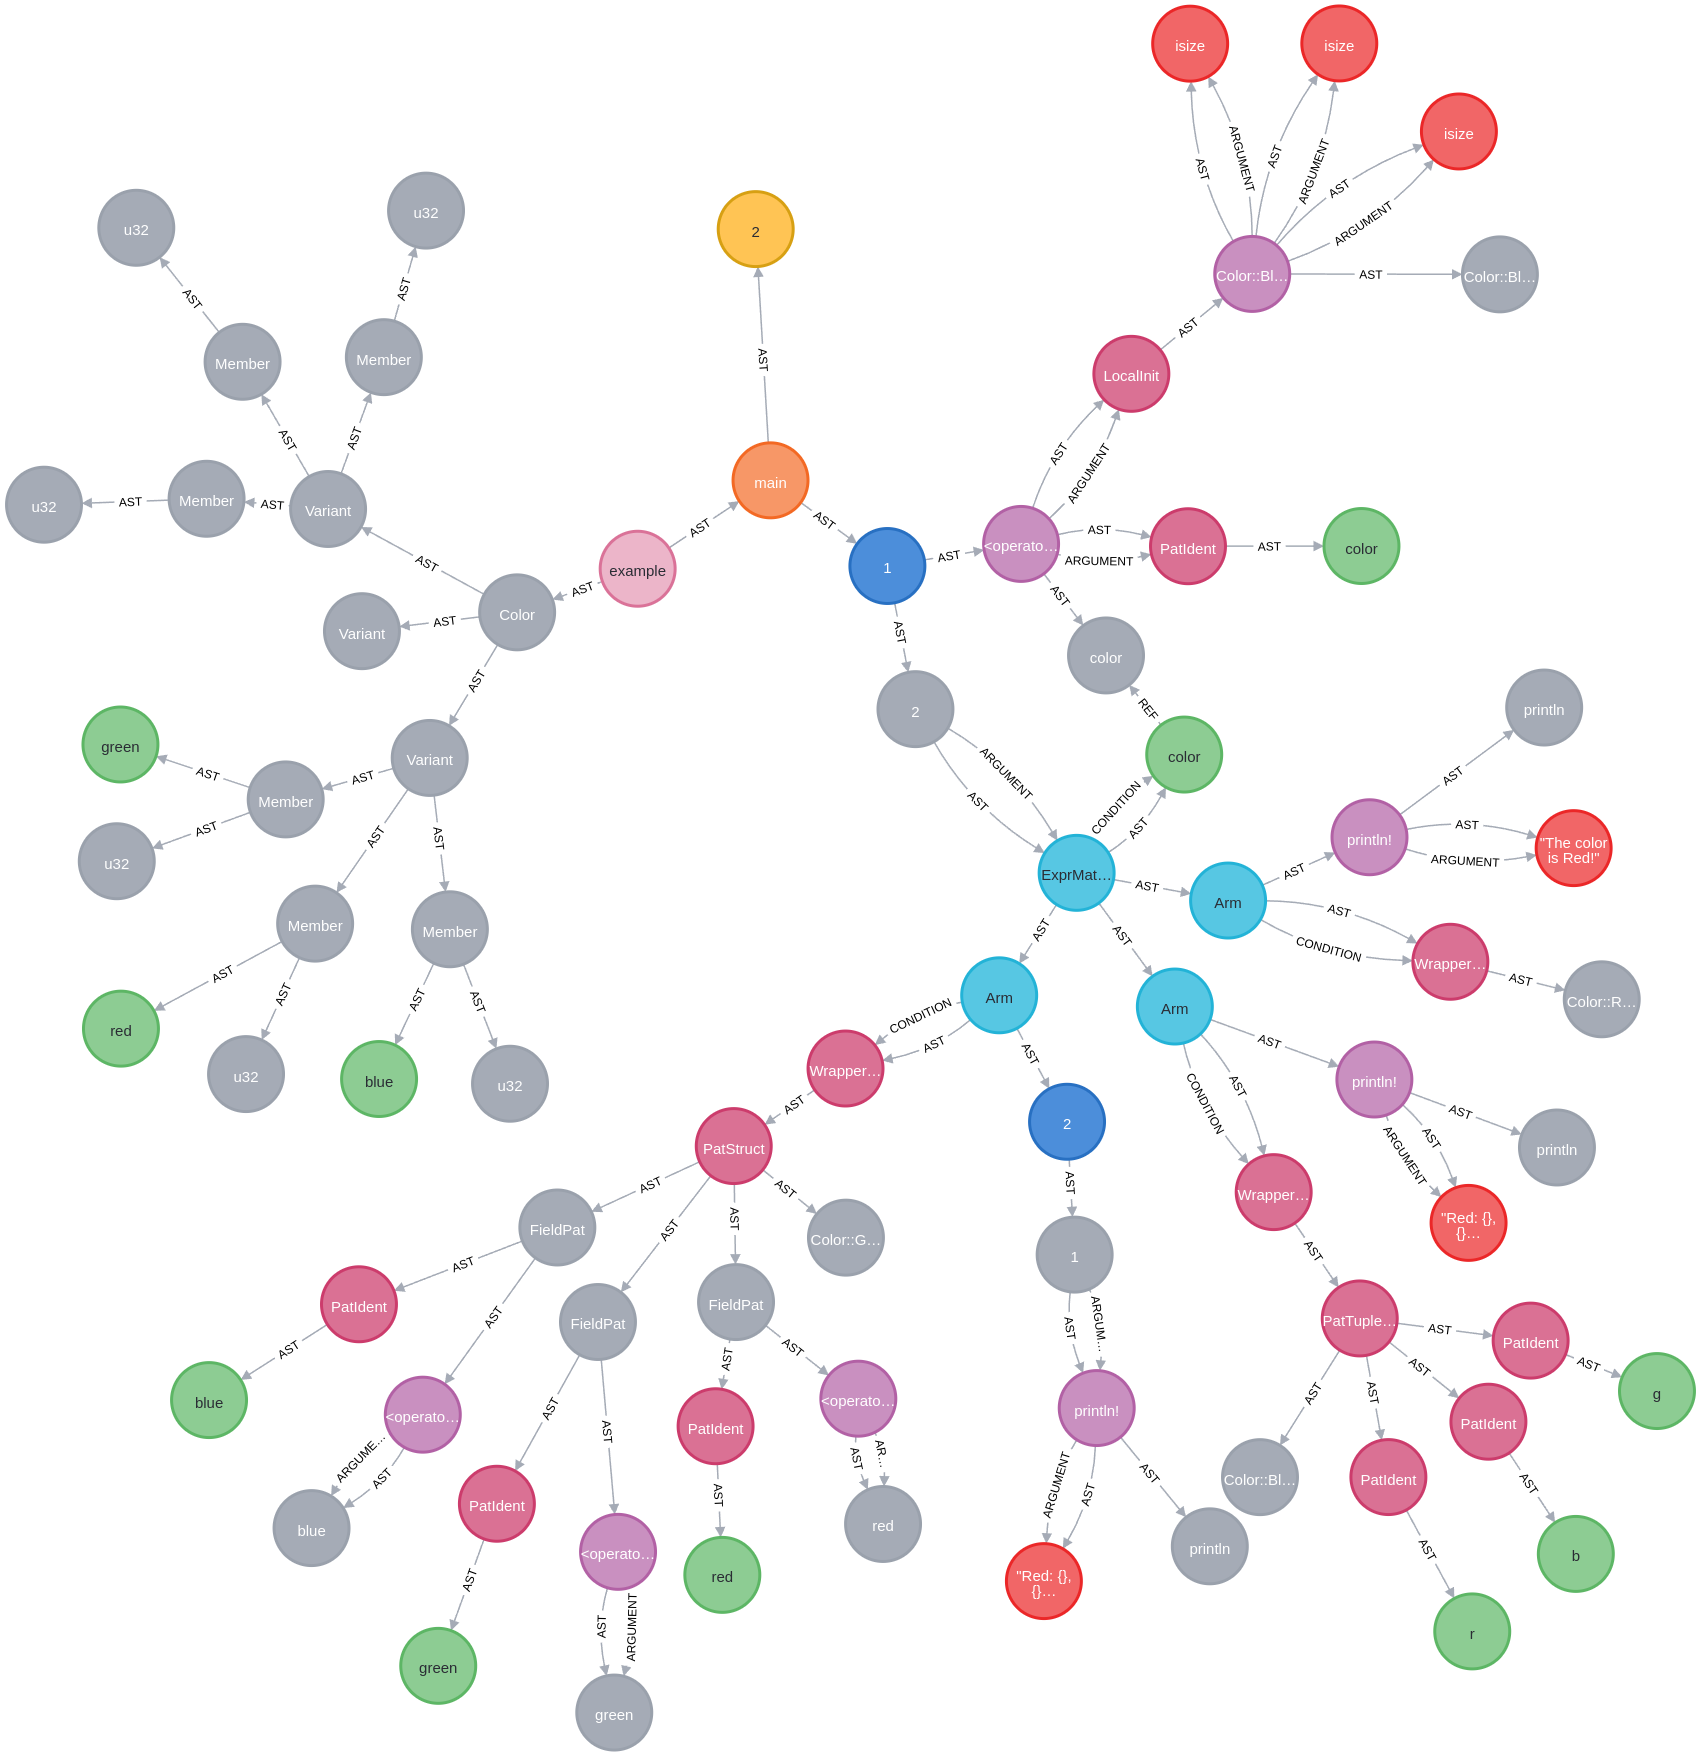
\includegraphics[width=1\columnwidth]{figures/c4/c4_match.png}
    \centering
    \caption{Minh họa đồ thị CPG cho đoạn mã nguồn cú pháp match \ref{code:c4_match}.}
    \label{img:c4_match}
\end{figure}

\subsection{Cú pháp lifetime}

Lifetime là cơ chế được sử dụng trong Rust để quản lý vòng đời của các biến tham chiếu.
Quản lý lifetime một cách chặt chẽ đảm bảo rằng các biến tham chiếu không trỏ tới vùng nhớ không còn tồn tại.
Lifetime có vai trò tương tự như kiểu tổng quát, nhưng thay vì định kiểu cho biến thì lifetime sẽ xác định thời gian hợp lệ cho biến tham chiếu.
Để biểu diễn được kiểu dữ liệu tổng quát, đặc tả CPG của Joern đã có các nút như \texttt{TYPE}, \texttt{TYPE PARAMETER}, \texttt{TYPE ARGUMENT}.
Do vậy để biểu diễn được tính năng lifetime trên đồ thị CPG, 3 loại nút mới đã được thêm vào đặc tả CPG bao gồm \texttt{LIFETIME}, \texttt{LIFETIME PARAMETER}, \texttt{LIFETIME ARGUMENT}.
Để chỉ ra quan hệ ràng buộc giữa biến và lifetime hay quan hệ giữa các lifetime với nhau, ta sẽ thêm cạnh \texttt{OUT LIVE}.
Cạnh \texttt{OUT LIVE} mang ý nghĩa nút nguồn phải có thời gian hợp lệ lớn hơn nút đích. Quy định về thời gian hợp lệ của một đơn vị thành phần so với đơn vị thành phần khác được tham khảo từ Rust Reference.

Nút \texttt{LIFETIME PARAMETER} và \texttt{LIFETIME ARGUMENT} được sử dụng cho các \texttt{struct}, \texttt{enum}, \texttt{trait} để chỉ ra lifetime tổng quát cho các biến tham chiếu.
Loại nút \texttt{LIFETIME} sẽ thể hiện vòng đời thực sự của biến tham chiếu.
Các biến tham chiếu sẽ được gán lifetime thông qua việc sử dụng dấu "\texttt{'}" đi trước tên lifetime, ví dụ như \texttt{'a}.
Nếu biến đánh dấu lifetime \texttt{'a} thì sẽ có cạnh \texttt{OUT LIVE} trỏ từ nút \texttt{IDENTIFIER} của biến tới nút \texttt{LIFETIME} đại diện cho \texttt{'a} tương ứng.
Nếu lifetime \texttt{'a} được giới hạn bởi lifetime \texttt{'b} thì sẽ có cạnh \texttt{OUT LIVE} từ nút \texttt{LIFETIME} \texttt{'a} tới nút \texttt{LIFETIME} \texttt{'b}.

% Lifetime elision là cơ chế trong Rust giúp tự động suy diễn lifetime cho các biến tham chiếu.
% Có ba luật chính về lifetime elision trong Rust.
% Thứ nhất, mỗi biến tham chiếu đầu vào sẽ được tự động gán lifetime mà không cần phải đánh dấu một cách tường minh.
% Thứ hai, nếu hàm có chỉ có một biến tham chiếu đầu và một biến tham chiếu đầu ra, trình biên dịch sẽ suy luận rằng biến tham chiếu đầu ra có cùng lifetime với biến tham chiếu đầu vào.
% Cuối cùng, nếu hàm có một hoặc nhiều hơn một biến tham chiếu đầu vào và một trong biến đầu vào là biến \texttt{self} (\texttt{self} tương đương với \texttt{this} trong C/C++), trình biên dịch sẽ suy luận rằng biến tham chiếu đầu ra có cùng lifetime với \texttt{self}.
% Ngoài 3 trường hợp trên, Rust yêu cầu phải ghi rõ lifetime cho tất cả các biến tham chiếu để tránh nhầm lẫn và đảm bảo an toàn bộ nhớ.

\begin{listing}[H]
\begin{minted}[mathescape, breaklines, frame=lines, framesep=2mm, baselinestretch=1.2, fontsize=\footnotesize, linenos]{rust}
fn longest<'a>(x: &'a str, y: &'a str) -> &'a str {
    if x.len() > y.len() {
        x
    } else {
        y
    }
}
\end{minted}
\caption{Ví dụ đoạn mã nguồn cho cú pháp lifetime.}
\label{code:c4_lifetime_1}
\end{listing}

Các biến tham chiếu luôn có một lifetime tương ứng với nó, có thể được chỉ ra tường minh hoặc không tường minh.
Đoạn mã \ref{code:c4_lifetime_1} mô tả một ví dụ bắt buộc phải khai báo lifetime một cách tường minh để chỉ rõ vòng đời của biến tham chiếu.
Hàm \texttt{longest} nhận vào 2 biến tham chiếu \texttt{x} và \texttt{y} cùng có lifetime \texttt{'a} và giá trị trả về cũng có lifetime \texttt{'a}.
Trình biên dịch Rust có thể tự động suy diễn lifetime không tường minh cho hai biến tham chiếu đầu vào \texttt{x} và \texttt{y}, nhưng không thể suy diễn được lifetime cho giá trị tham chiếu trả về.
Hơn nữa, giá trị trả về của hàm \texttt{longest} là một trong hai giá trị tham chiếu đầu vào.
Do trình biên dịch không thể biết được trong khi thực thi hàm thì giá trị trả về sẽ trỏ tới vùng nhớ của \texttt{x} hay \texttt{y}, do đó cần phải chỉ rõ lifetime cho giá trị trả về.
Biến \texttt{x} và \texttt{y} cùng có lifetime \texttt{'a} tức là \texttt{x} và \texttt{y} sẽ có một khoảng thời gian mà \texttt{x} và \texttt{y} cùng tồn tại và đặt tên khoảng thời gian đó là \texttt{'a}.
Giá trị đầu ra tồn tại trong khoảng thời gian \texttt{'a} này thì luôn đảm bảo không trỏ tới vùng nhớ không còn tồn tại.
Khi sử dụng hàm, nếu đối số đầu vào hay biến nhận giá trị trả về không thỏa mãn ràng buộc lifetime \texttt{'a} thì trình biên dịch Rust sẽ báo lỗi.

\vspace{\baselineskip}

\begin{figure}[H]
    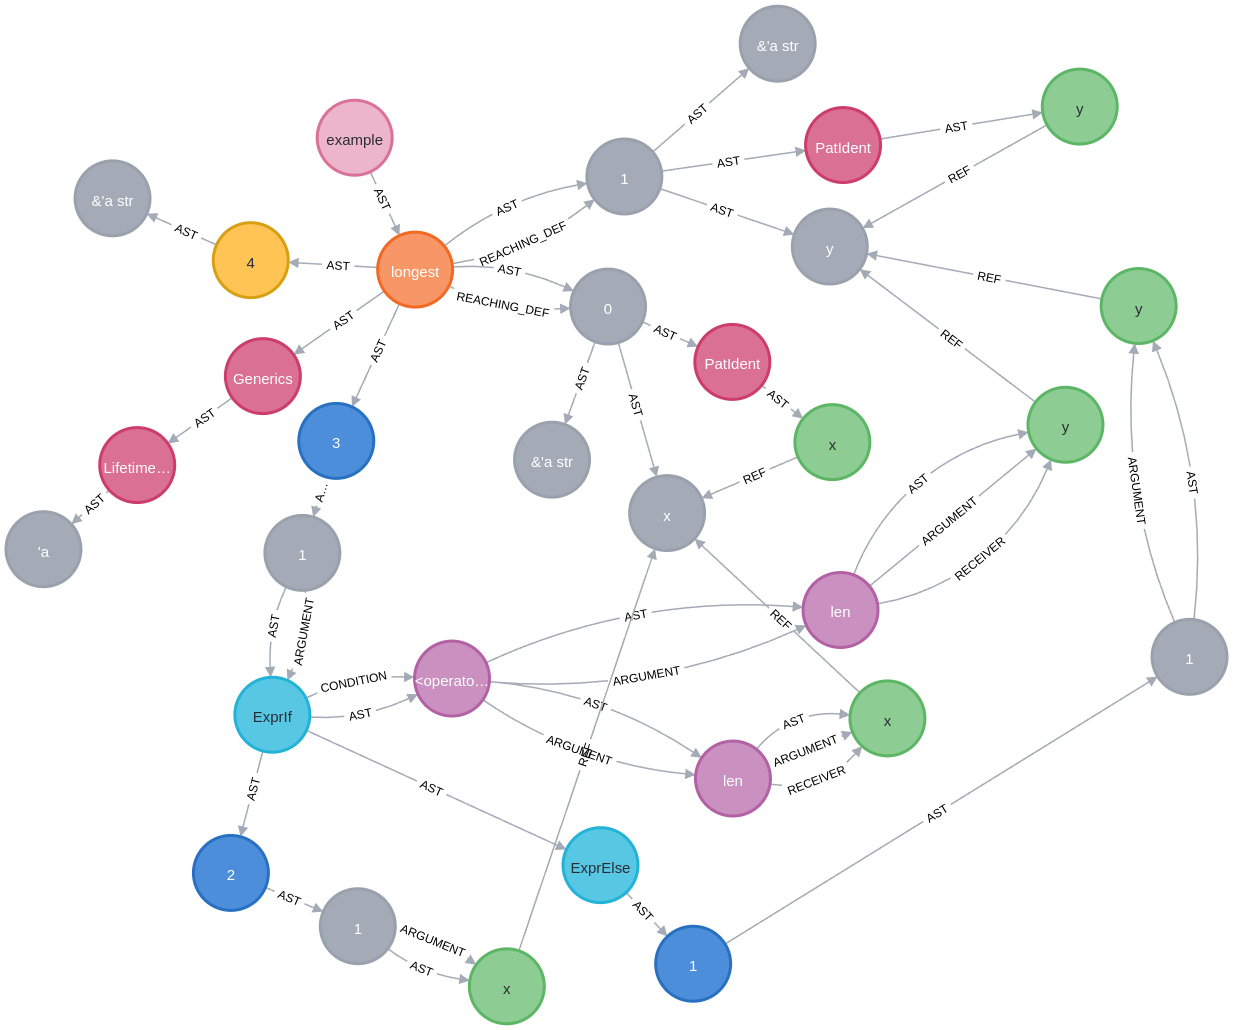
\includegraphics[width=1\columnwidth]{figures/c4/c4_lifetime_1.png}
    \centering
    \caption{Minh họa đồ thị CPG cho đoạn mã nguồn cú pháp lifetime \ref{code:c4_lifetime_1}.}
    \label{img:c4_lifetime_1}
\end{figure}

Hình \ref{img:c4_lifetime_1} thể hiện mối quan hệ lifetime giữa các biến tham chiếu và giá trị trả về của hàm.
Hàm \texttt{longest} được thể hiện qua nút \texttt{METHOD}.
Trong đó, nút \texttt{METHOD} có cạnh \texttt{AST} trỏ tới nút \texttt{GENERICS}, đại diện cho nút cha bọc lấy nhiều nút thể hiện kiểu tổng quát.
Nút \texttt{LIFETIME PARAMETER} thể hiện lifetime \texttt{'a} của hàm, và cũng là lifetime của các biến tham chiếu và giá trị trả về.
Các biến tham chiếu \texttt{x} và \texttt{y} có cùng lifetime \texttt{'a} được thể hiện qua cạnh \texttt{OUT LIVE} từ nút \texttt{IDENTIFIER} của biến \texttt{x} và \texttt{y} tới nút \texttt{LIFETIME} của \texttt{'a}.
Giá trị trả về của hàm cũng có lifetime \texttt{'a} và được thể hiện qua cạnh \texttt{OUT LIVE} từ nút \texttt{METHOD RETURN} tới nút \texttt{LIFETIME} \texttt{'a}.
Mối quan hệ lifetime giữa các biến tham chiếu và giá trị trả về đều được thể hiện qua các nút \texttt{LIFETIME} và cạnh \texttt{OUT LIVE} trên đồ thị CPG.

\begin{listing}[H]
\begin{minted}[mathescape, breaklines, frame=lines, framesep=2mm, baselinestretch=1.2, fontsize=\footnotesize, linenos]{rust}
fn f<'a, 'b, 'c, T>(x: &'a i32, mut y: &'b i32, z: &'c T)
where
    'b: 'a,
    'c: 'b,
    T: 'b,
{
    // ...
}
\end{minted}
\caption{Ví dụ đoạn mã nguồn cho cú pháp lifetime kết hợp cú pháp where.}
\label{code:c4_lifetime_2}
\end{listing}


\begin{figure}[H]
    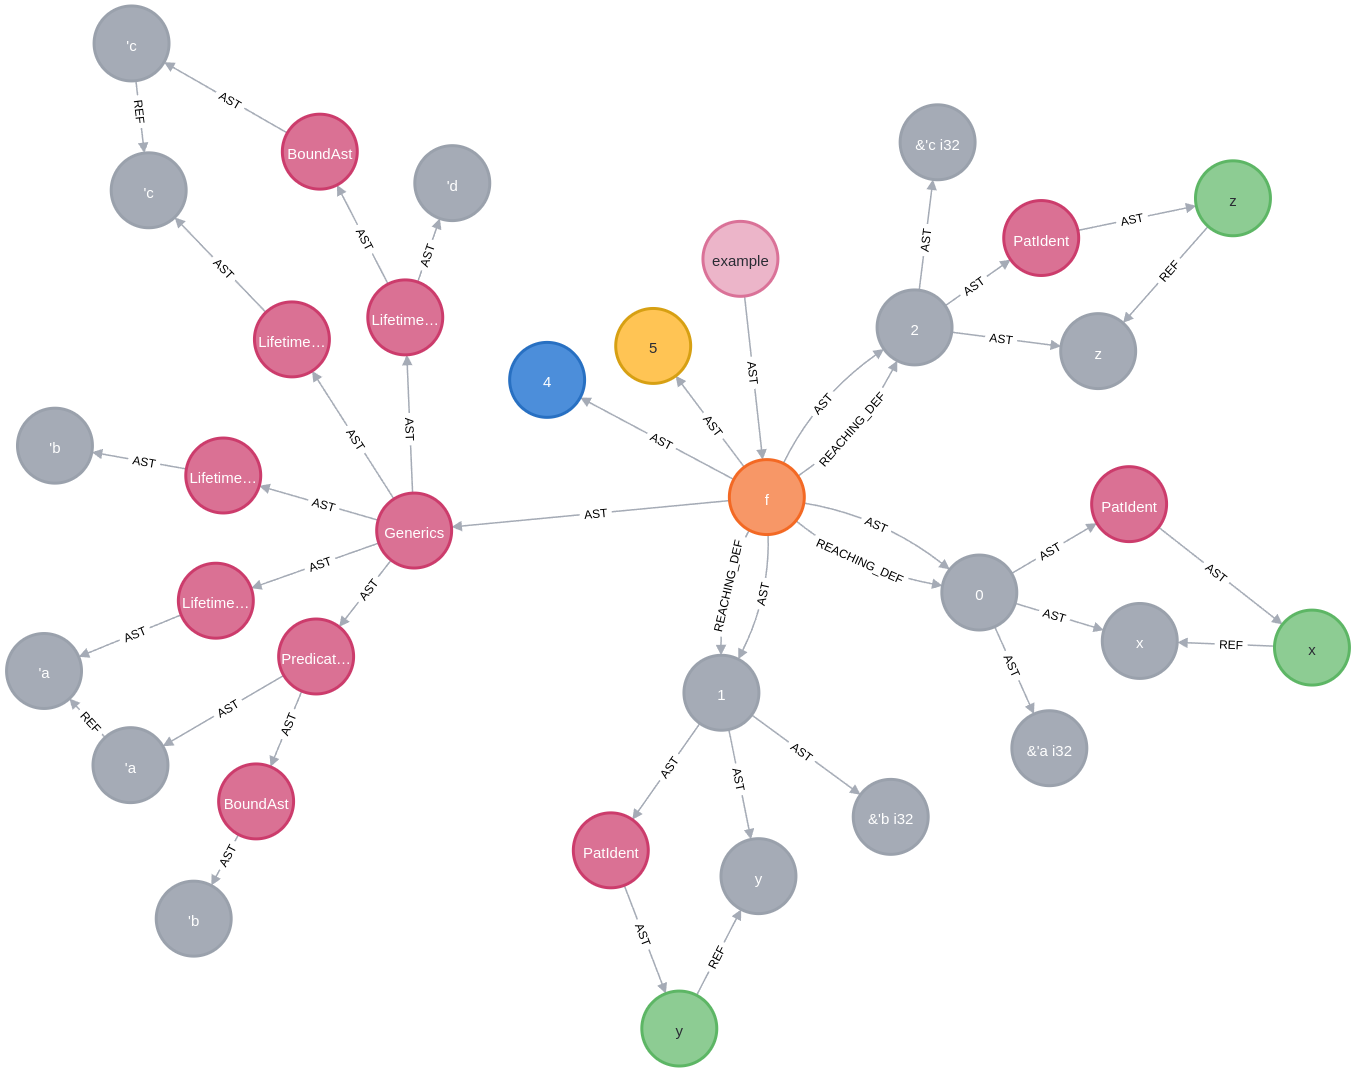
\includegraphics[width=1\columnwidth]{figures/c4/c4_lifetime_2.png}
    \centering
    \caption{Minh họa đồ thị CPG cho đoạn mã nguồn cú pháp where \ref{code:c4_lifetime_2}.}
    \label{img:c4_lifetime_2}
\end{figure}

Trong Rust, kiểu tổng quát và ràng buộc của nó có thể được chỉ rõ thông qua cú pháp \texttt{where}.
Cú pháp \texttt{where} cho phép thể hiện ràng buộc giữa kiểu dữ liệu tổng quát và kiểu lifetime tổng quát.
Đoạn mã \ref{code:c4_lifetime_2} minh họa về một hàm có nhiều lifetime, nhiều kiểu tổng quát và tham chiếu đầu vào kết hợp với cú pháp \texttt{where} để thể hiện mối quan hệ ràng buộc giữa chúng.
Hàm \texttt{f} nhận vào 3 biến tham chiếu \texttt{x}, \texttt{y}, \texttt{z} có lifetime tương ứng là \texttt{'a}, \texttt{'b}, \texttt{'c}.
Cú pháp \texttt{'b: 'a} thể hiện ràng buộc lifetime \texttt{'b} của biến \texttt{y} phải lớn hơn hoặc bằng lifetime \texttt{'a} của biến \texttt{x}.
Trên đồ thị CPG ở Hình \ref{img:c4_lifetime_2}, điều này tức là sẽ có cạnh \texttt{OUT LIVE} từ nút \texttt{LIFETIME} \texttt{'b} tới nút \texttt{LIFETIME} \texttt{'a}.
Điều này tương tự với việc lifetime \texttt{'c} của biến \texttt{z} phải lớn hơn hoặc bằng lifetime \texttt{'b} của biến \texttt{y}.
Cạnh \texttt{OUT LIVE} từ nút \texttt{LIFETIME} \texttt{'c} tới nút \texttt{LIFETIME} \texttt{'b} được thể hiện rõ ràng trên đồ thị CPG.

Không chỉ ràng buộc giữa các lifetime với nhau, hoàn toàn có thể ràng buộc lifetime cho một kiểu dữ liệu tổng quát.
Kiểu dữ liệu \texttt{T} của biến \texttt{z} phải có lifetime lớn hơn \texttt{'c} thông qua cú pháp \texttt{T: 'c}.
Cú pháp này sẽ có ý nghĩa trong trường hợp khi T là một kiểu \texttt{struct} tự định nghĩa, thì tất cả các thuộc tính tham chiếu của T cũng phải có lifetime lớn hơn hoặc bằng \texttt{'c}.
Sẽ có cạnh \texttt{LIFETIME} từ nút \texttt{TYPE} của kiểu \texttt{T} tới nút \texttt{LIFETIME} \texttt{'c} để thể hiện mối quan hệ ràng buộc giữa chúng.
Rust cung cấp hai cách để thể hiện ràng buộc cho kiểu dữ liệu và kiểu lifetime tổng quát.
Một là khai báo ngay tại phần khai báo hàm, hai là sử dụng cú pháp \texttt{where} để thể hiện ràng buộc.
Lưu ý rằng khai báo ngay tại hàm và cú pháp \texttt{where} không thay thế cho nhau mà cùng tồn tại để có thể kết hợp với nhau.
Khai báo ngay tại hàm mang ý nghĩa khai báo nên sẽ sử dụng các nút \texttt{TYPE PARAMETER} và \texttt{LIFETIME PARAMETER} để thể hiện.
Còn cú pháp \texttt{where} mang ý nghĩa ràng buộc nên sẽ sử dụng nút \texttt{LIFETIME}, cạnh \texttt{OUT LIVE}, cạnh \texttt{REF}.

Ownership, borrowing và lifetime là 3 tính năng làm nên cơ chế an toàn bộ nhớ trong Rust.
Đây là bộ ba tính năng quan trọng làm cho Rust trở nên khác biệt so với các ngôn ngữ lập trình khác.
Đồ thị CPG cần phải thể hiện được 3 tính năng trên và cung cấp thông tin thông qua các nút, cạnh và thuộc tính phù hợp.
Đặc biệt là tính năng lifetime thể hiện sự hợp lệ của các biến tham chiếu.
Do đó việc thể hiện đúng quan hệ giữa lifetime và biến, lifetime với lifetime, biến với biến là rất quan trọng.
Từ đó có thể khai thác thông tin để kiểm tra sự hợp lệ của biến tham chiếu, giúp phát hiện được các lỗi về bộ nhớ gây ra khi đánh dấu lifetime không chính xác.
